\documentclass[conference,table]{IEEEtran}
\IEEEoverridecommandlockouts
% The preceding line is only needed to identify funding in the first footnote. If that is unneeded, please comment it out.
\usepackage{cite}
\usepackage{amsmath,amssymb,amsfonts}
\usepackage{algorithmic}
\usepackage{array}
\usepackage{gensymb}
\usepackage{graphicx}
\usepackage{multirow}
\usepackage{pgfplots}
\usepackage{tabularx}
\usepackage{textcomp}
\def\BibTeX{{\rm B\kern-.05em{\sc i\kern-.025em b}\kern-.08em
		T\kern-.1667em\lower.7ex\hbox{E}\kern-.125emX}}
\begin{document}
	
	\title{Classification of Fruits and Vegetables on a Conveyor}
	\author{
		\IEEEauthorblockN{Arvind Suresh, Sriram Suresh, Enoch Ramesh}
		\IEEEauthorblockA{\textit{University of Waterloo}\\
			Waterloo, Canada \\
			a7suresh/s9suresh/eramesh@edu.uwaterloo.ca}
	}
	
	\maketitle
	
	\begin{abstract}
		The aim of this paper is to develop a method to quickly and efficiently identify different types of fruits and vegetables that are travelling on a conveyor. Twenty four different categories of fruits and vegetables, with 80 images per category, are used for training. Segmentation is first performed on the images with two segmentation masks, which are then downsampled using max-pooling to 25\% of the original size. The masked images before downsampling are used with local binary patterns (LBP) and histogram oriented gradients (HOG) feature extraction methods to get the textures and shapes. Principal component analysis (PCA) is performed on the downsampled image and extracted features to reduce the number of principal components such that 95\% of the initial variance is maintained. Finally, these are fed into the classifier to identify the category of fruit or vegetable. Classification is tested using two classifiers: bagged decision tree and boosted support vector machine (SVM). The results show that the bagged decision tree classifier has a higher accuracy than the boosted SVM classifier. Furthermore, the classification is done with a high degree of accuracy.
	\end{abstract}
	
	\begin{IEEEkeywords}
		Fruit classification, vegetable classification, image classification, image segmentation, max-pooling, feature extraction, local binary patterns (LBP), histogram oriented gradients (HOG), bagging, decision tree, boosting, support vector machine (SVM)
	\end{IEEEkeywords}
	
	\section{Introduction}
	Economic growth, increasing global per capita incomes, and rising consumer spending are all contributing to a boom in demand for a huge number of consumer products and other commodities. Fruit and vegetable industries are no exception \cite{b1_1}. However, with increasing demand comes increasing challenges for producers and processors. Some challenges are far from unique to this sector, such as growing competition \cite{b1_2} and environmental concerns \cite{b1_3}. Unlike many products though, fruits and vegetables face the imminent threat of spoilage and need to be handled and processed quickly, which puts a great burden on production lines to be quick and effective. Conveyor belts are used extensively for this reason to perform tasks such as sorting, washing, and packaging fruits and vegetables \cite{b1_4}. Machine learning (ML) can be used to classify different types of fruits and vegetables travelling on a conveyor to further aid in some aspects, such as inventory tracking and sorting.

Deep neural networks (DNNs) have advanced to encompass various areas of problems \cite{b1_5,b1_6}. However, due to the ability to have a large number of hidden layers \cite{b1_7}, DNNs can become computationally intensive and time consuming to train and run \cite{b1_8}. $\langle$ Placeholder text for methods used in this paper $\rangle$

$\langle$ Placeholder text for results $\rangle$
	
	\section{Related Literature}
	In the agriculture field, remote sensing with intelligent processing (RSIP) technologies are used for monitoring purposes \cite{b2_1}. This has also been extended to classification with the use of polarimetry synthetic aperture Radar (PolSAR). PolSAR has had plenty of successful applications in various fields in the past \cite{b2_2,b2_3,b2_4}, including crop classification and monitoring \cite{b2_5,b2_6}. PolSAR can obtain polarimetric information through the use of electromagnetic waves and has become one of the mainstreams in microwave remote sensing. For crop classification, polarimetric features, augmented with multi-temporal data, is used with a deep convolutional neural network (CNN) to achieve high accuracies with a low amount of training samples \cite{b2_7}.

Other classification techniques have been developed and used in the area of fruits and vegetables. In applications such as grading fruits and other agricultural products, features such as size, shape, colour and texture are used \cite{b2_8,b2_9,b2_10}. Accuracy is improved through the use of incorporating depth when capturing red-green-blue (RGB) images. The use of RGB-depth (RGB-D) images and CNNs have been demonstrated to be excellent for classification and recognition tasks \cite{b2_11,b2_12}, including fruits and vegetables \cite{b2_13}.

While deep CNNs are the most predominantly used method in applications of single and multiple types of vegetable classification \cite{b2_14,b2_15,b2_16}, some examples that are part of bigger systems such as farm robots \cite{b2_17} or smart fridges \cite{b2_18} have successfully employed feature extraction methods such as local binary patterns (LBP) and histogram oriented gradients (HOG) \cite{b2_19,b2_20}. In this paper, we propose augmenting the image data with LBP feature extraction to use with fast classifiers.
	
	\section{Data Acquisition} \label{daq}
	For the validation of the proposed feature augmented classifier, we create a dataset of 30 fruits and vegetables (see Table \ref{tab:veg_types}). We capture 10 RGB images for each type of fruit or vegetable. Each of these images are rotated 7 times to create new images, resulting in a total of 2400 RGB images for training.

\bgroup
\def\arraystretch{1.5}
\begin{table}[htbp]
	\caption{Types of Fruits and Vegetables Used for Creating the Dataset}
	\begin{center}
		\begin{tabular}{| >{\centering\arraybackslash}m{2cm} | >{\centering\arraybackslash}m{2cm} | >{\centering\arraybackslash}m{2cm} |}
			\hline
			Cabbage & White Turnip & \\
			\hline
			Tomato & Okra & \\
			\hline
			Orange Pepper & Eggplant & \\
			\hline
			Red Pepper & Squash Zucchini & \\
			\hline
			Jalapeno & Carrot & \\
			\hline
			Green Pepper & & \\
			\hline
			Beet & & \\
			\hline
			Daikon Lo Bok & & \\
			\hline
			Bok Choi & & \\
			\hline
			Brussel Sprout & & \\
			\hline
		\end{tabular}
		\label{tab:veg_types}
	\end{center}
\end{table}
\egroup

As Fig. \ref{fig:veg_rotations} shows, the 7 rotations are applied at increasing increments of 45\degree{} starting from the original. We do this to account for non-symmetric fruits and vegetables that are not axis aligned.

\bgroup
\def\arraystretch{1.5}
\begin{figure*}[tp]
	\begin{center}
		\begin{tabular}{c|ccccccc}
			Original & \multicolumn{7}{c}{Rotated} \\
			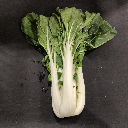
\includegraphics[scale=0.4]{./img/bokchoi_0.png} &
			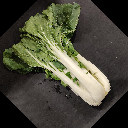
\includegraphics[scale=0.4]{./img/bokchoi_1.png} &
			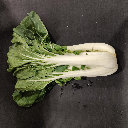
\includegraphics[scale=0.4]{./img/bokchoi_2.png} &
			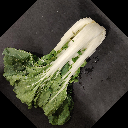
\includegraphics[scale=0.4]{./img/bokchoi_3.png} &
			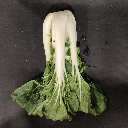
\includegraphics[scale=0.4]{./img/bokchoi_4.png} &
			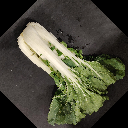
\includegraphics[scale=0.4]{./img/bokchoi_5.png} &
			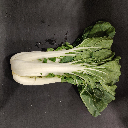
\includegraphics[scale=0.4]{./img/bokchoi_6.png} &
			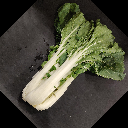
\includegraphics[scale=0.4]{./img/bokchoi_7.png} \\
			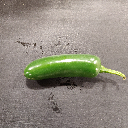
\includegraphics[scale=0.4]{./img/jalapeno_0.png} &
			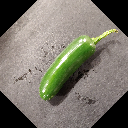
\includegraphics[scale=0.4]{./img/jalapeno_1.png} &
			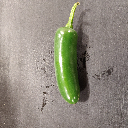
\includegraphics[scale=0.4]{./img/jalapeno_2.png} &
			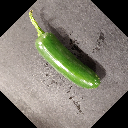
\includegraphics[scale=0.4]{./img/jalapeno_3.png} &
			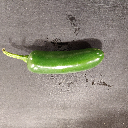
\includegraphics[scale=0.4]{./img/jalapeno_4.png} &
			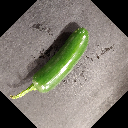
\includegraphics[scale=0.4]{./img/jalapeno_5.png} &
			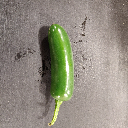
\includegraphics[scale=0.4]{./img/jalapeno_6.png} &
			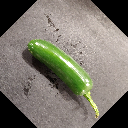
\includegraphics[scale=0.4]{./img/jalapeno_7.png} \\
			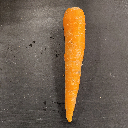
\includegraphics[scale=0.4]{./img/carrot_0.png} &
			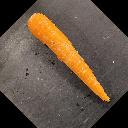
\includegraphics[scale=0.4]{./img/carrot_1.png} &
			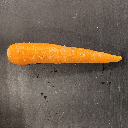
\includegraphics[scale=0.4]{./img/carrot_2.png} &
			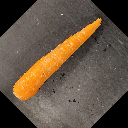
\includegraphics[scale=0.4]{./img/carrot_3.png} &
			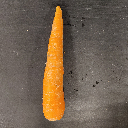
\includegraphics[scale=0.4]{./img/carrot_4.png} &
			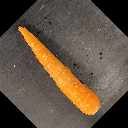
\includegraphics[scale=0.4]{./img/carrot_5.png} &
			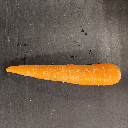
\includegraphics[scale=0.4]{./img/carrot_6.png} &
			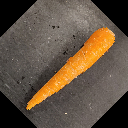
\includegraphics[scale=0.4]{./img/carrot_7.png} \\
			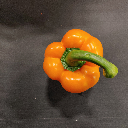
\includegraphics[scale=0.4]{./img/pepper_0.png} &
			
\includegraphics[scale=0.4]{./img/pepper_1.png} &
			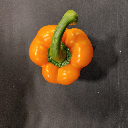
\includegraphics[scale=0.4]{./img/pepper_2.png} &
			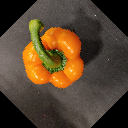
\includegraphics[scale=0.4]{./img/pepper_3.png} &
			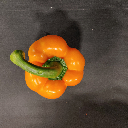
\includegraphics[scale=0.4]{./img/pepper_4.png} &
			
\includegraphics[scale=0.4]{./img/pepper_5.png} &
			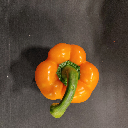
\includegraphics[scale=0.4]{./img/pepper_6.png} &
			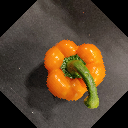
\includegraphics[scale=0.4]{./img/pepper_7.png} \\
		\end{tabular}
		\label{tab:veg_types}
	\end{center}
	\caption{Four sample images with their rotated counterparts.}
	\label{fig:veg_rotations}
\end{figure*}
\egroup
	
	\section{Image Preprocessing} \label{preprocessing}
	\subsection{Image Segmentation}
Image segmentation is an effective means of isolating an object from its background and has been successfully used for different applications \cite{b4_1,b4_2,b4_3}. We perform segmentation with 2 segmentation masks -- one for brighter vegetables and one for darker vegetables. The values for the masks (see Table \ref{tab:mask_vals}) are selected experimentally based on their performances on the training images.

\bgroup
\def\arraystretch{1.5}
\begin{table}[htbp]
	\caption{Treshold Values for Segmentation Masks}
	\begin{center}
		\begin{tabular}{|c|c|c|c|c|}
			\hline
			& \multicolumn{4}{c|}{\textbf{Colour}}                                                         \\ \cline{2-5} 
			\multirow{-2}{*}{\textbf{Mask}} & \multicolumn{2}{c|}{\textbf{Lower Treshold}} & \multicolumn{2}{c|}{\textbf{Upper Treshold}}  \\ \hline
			Light Vegetable Mask            & RGB(0, 40, 40)   & \cellcolor[HTML]{002828}  & RGB(240, 240, 240) & \cellcolor[HTML]{F0F0F0} \\ \hline
			Dark Vegetable Mark             & RGB(0, 80, 80)   & \cellcolor[HTML]{005050}  & RGB(255, 255, 255) & \cellcolor[HTML]{FFFFFF} \\ \hline
		\end{tabular}
		\label{tab:mask_vals}
	\end{center}
\end{table}
\egroup

Once the two masks are applied to an image, they are downsampled with max-pooling to 25\% of the original size as illustrated in Fig. \ref{fig:mask}. We do this to reduce the computational complexity of learning and to make the model more tolerant to slight displacements. The resultant image is used as an input for the classifiers discussed in section \ref{classifiers}.

\begin{figure}[tp]
	\centerline{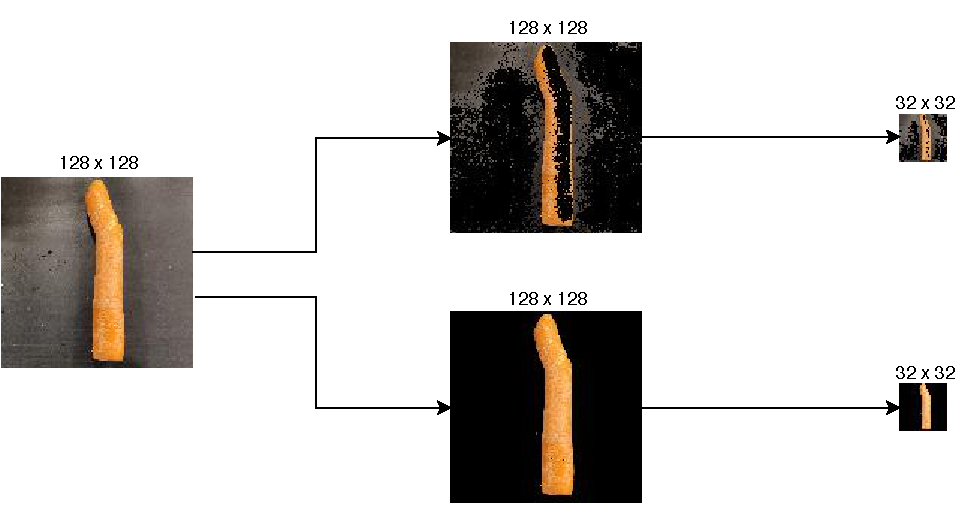
\includegraphics[scale=0.5]{./img/mask.pdf}}
	\caption{The steps to extract masked downsampled data.}
	\label{fig:mask}
\end{figure}

\subsection{Feature Extraction}
In addition to segmentation, additional attributes and characteristics of the vegetables are extracted with feature extraction methods \cite{b4_4}. We use LBP and HOG to get the textures and shapes of the vegetables respectively. As shown in Fig. \ref{fig:lbp_hog}, both feature extractions are applied to the 2 masked images before they are max-pooled. We do this to retain a high quality for feature extraction while focusing on only the object of interest without its background.

\begin{figure}[tp]
	\centerline{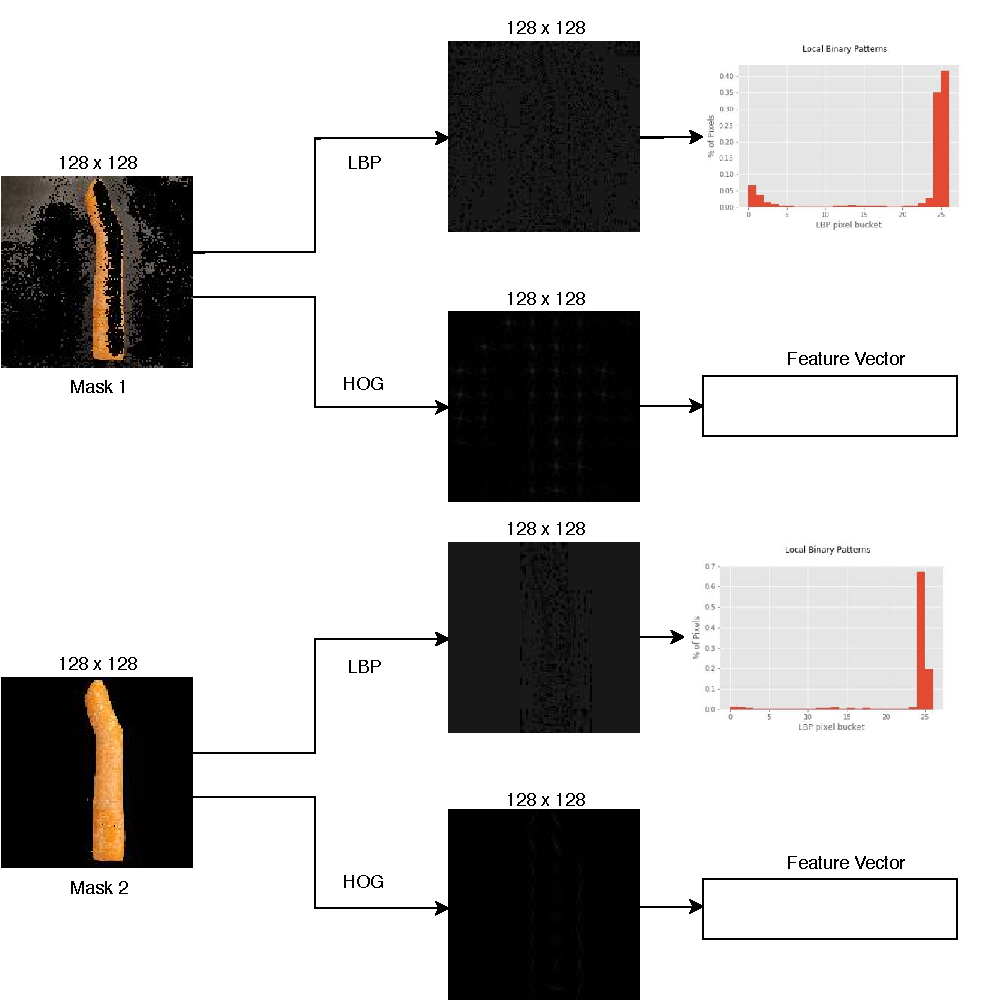
\includegraphics[scale=0.5]{./img/lbp_hog.pdf}}
	\caption{The steps to extract LBP and HOG feature vectors.}
	\label{fig:lbp_hog}
\end{figure}
	
	\section{Classification} \label{classifiers}
	The final stage is the classification stage. The inputs to this stage are the max-pooled masked images and feature vectors described in section \ref{preprocessing}. However, instead of using this as a direct input for classification, we reduce this data further as our objective is to reduce computational complexity and get a good runtime.

Principal component analysis (PCA) is a data transformation technique used to reduce the dimensionality of high-dimensional data into a low-dimensional subspace while maintaining most of the variance \cite{b5_1,b5_2}. The use of PCA to reduce the inputs to maintain most of the variance is a possibility if it doesn't result in a drastic drop in accuracy. The reduced data can be used as the input for classification as illustrated in Fig. \ref{fig:pca}.

We investigate using an ensemble classifier to compare accuracy. The ensemble method is a powerful technique that combines multiple models into a single predictive model. This often makes it more accurate and reliable than its individual components \cite{b5_3}. The classifier we propose is a decision tree classifier wrapped in a bagging based ensemble model. The bagging method selects a random subset of the dataset with replacements for training each model and uses a voting scheme to make a final prediction \cite{b5_4}. One of the more prominent examples of a bagged decision tree model is random forest \cite{b5_5}.

\begin{figure}[tp]
	\centerline{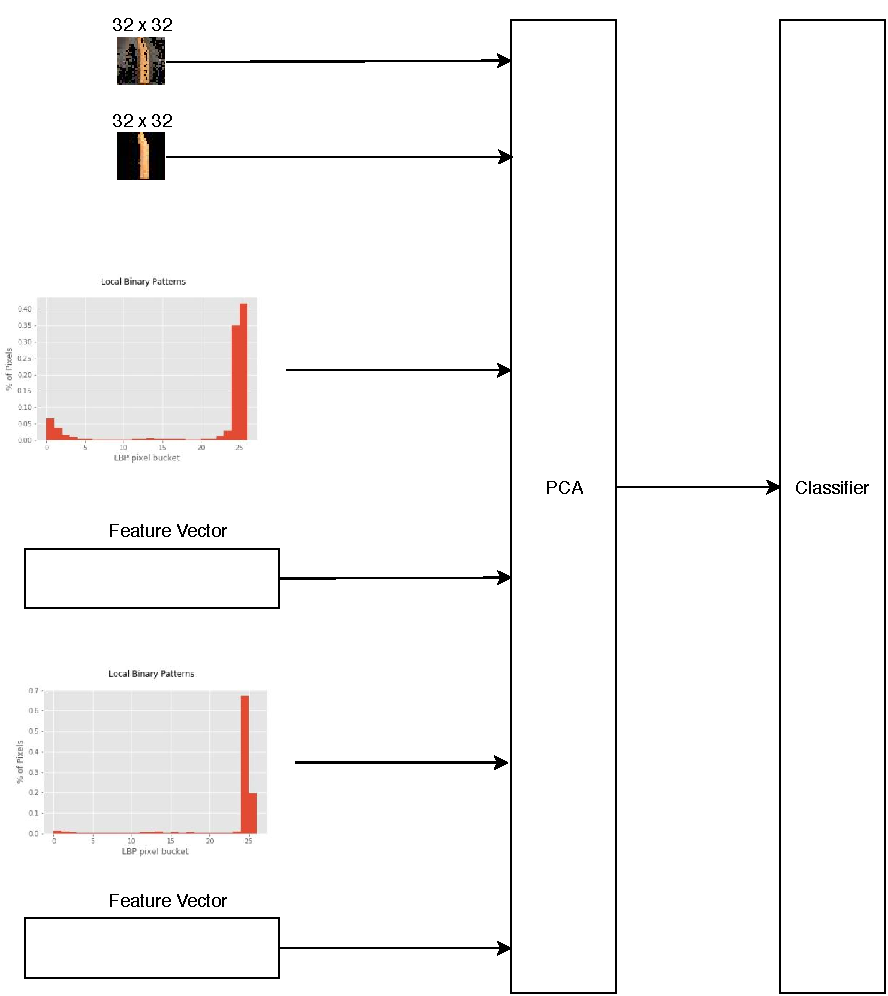
\includegraphics[scale=0.5]{./img/pca.pdf}}
	\caption{The steps to transform the input before classification.}
	\label{fig:pca}
\end{figure}
	
	\section{Results}
	The proposed system is implemented and evaluated using the 1920 RGB images described in section \ref{daq}. The first result that is evaluated is the effect of PCA on the accuracy of the classifier. We use 5-fold cross validation on a bagged decision tree ensemble with 25 trees as a starting point. This is used to compare the accuracies of using the unreduced input, PCA reduction to maintain 99\% variance and PCA reduction to maintain 95\% variance. As shown in Table \ref{tab:pca_comp}, the drop in accuracy is over 10\%, which is not acceptable for an application of this nature. Therefore, from this point on, no PCA is used.

\bgroup
\def\arraystretch{1.5}
\begin{table}[htbp]
	\caption{5-Fold Cross Validation Accuracies of Various PCA Levels}
	\begin{center}
		\begin{tabular}{|l|>{\centering\arraybackslash}m{1.75cm}|>{\centering\arraybackslash}m{1.75cm}|>{\centering\arraybackslash}m{1.75cm}|}
			\hline
			& \textbf{No PCA} & \textbf{99\% Variance PCA} & \textbf{95\% Variance PCA} \\
			\hline
			\# \textbf{Components} & 12596 & 1234 & 700 \\
			\hline
			\textbf{Accuracy} & 99.0625\% & 87.2917\% & 89.4792\% \\
			\hline
		\end{tabular}
		\label{tab:pca_comp}
	\end{center}
\end{table}
\egroup

The objective is to reduce computational complexity and get a good runtime. Thus, more trees than necessary should not be used in the ensemble classifier. To find the optimal number of trees, we perform 5-fold cross validation while varying the number of trees. From the result, shown in Fig. \ref{fig:num_trees}, some fluctuation in accuracy is shown when increasing the tree count past 7. However, this is likely due to the data being split up randomly when performing 5-fold cross validation. Therefore, it is safe to assume that the accuracy is fairly constant past 5 trees. This leads us to select 5 trees as the optimal number of trees.

\begin{figure}[tp]
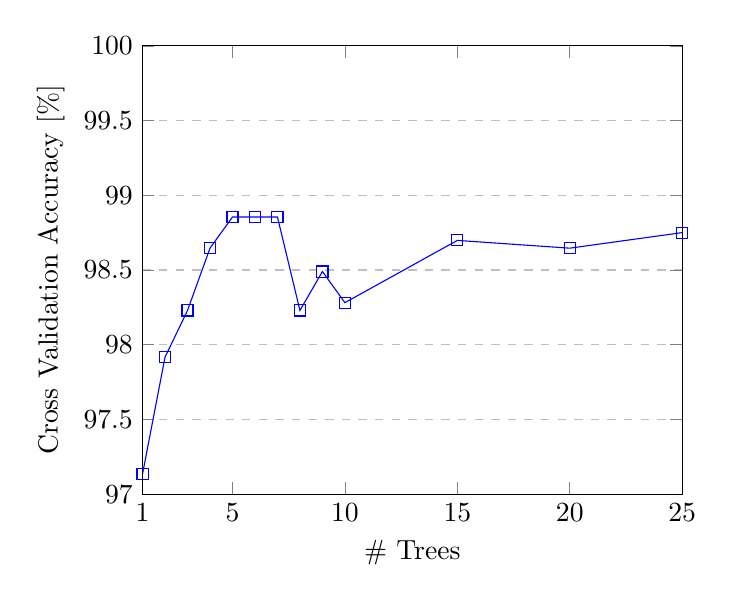
\begin{tikzpicture}
\begin{axis}[
xlabel={\# Trees},
ylabel={Cross Validation Accuracy [\%]},
xmin=1, xmax=25,
ymin=97, ymax=100,
xtick={1,5,10,15,20,25},
ytick={97.0,97.5,98.0,98.5,99.0,99.5,100.0},
ymajorgrids=true,
grid style=dashed,
]

\addplot[
color=blue,
mark=square,
]
coordinates {
	(1,97.1354)(2,97.9167)(3,98.2292)(4,98.6458)(5,98.8542)(6,98.8542)(7,98.8542)(8,98.2292)(9,98.4896)(10,98.2812)(15,98.6979)(20,98.6458)(25,98.75)
};

\end{axis}
\end{tikzpicture}
\caption{The effect of the number of trees on 5-fold cross validation accuracy.}
\label{fig:num_trees}
\end{figure}

To verify that this is indeed a good model all-round and is tolerant to different data-sizes, we perform k-fold cross validation varying k. The result, shown in Fig. \ref{fig:k_fold}, confirms the constancy of the classifier. Finally, we compare the accuracy and runtime of our classifier with Inception (see Table \ref{tab:inception_comp}), an established and successful DNN \cite{b6_1}. While the accuracy of our classifier is slighly lower than that of Inception, its runtime is significantly faster, proving to be a viable alternative.

\begin{figure}[tp]
	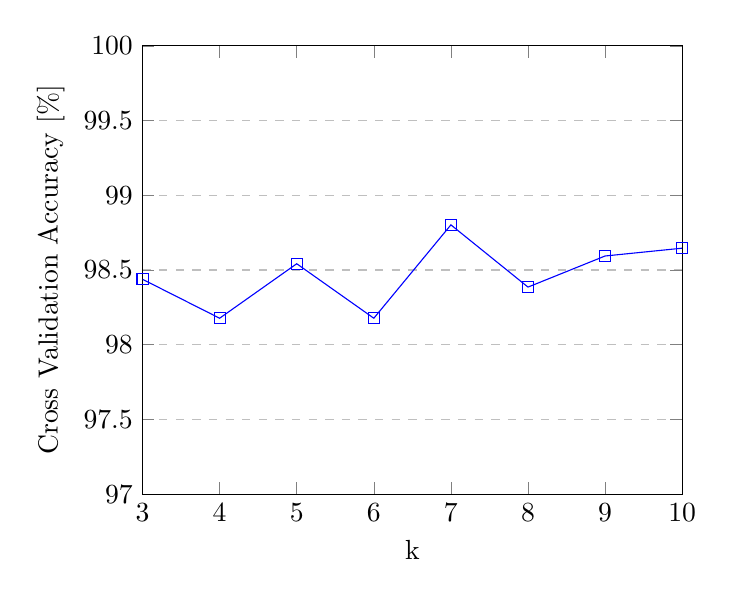
\begin{tikzpicture}
	\begin{axis}[
	xlabel={k},
	ylabel={Cross Validation Accuracy [\%]},
	xmin=3, xmax=10,
	ymin=97, ymax=100,
	xtick={3,4,5,6,7,8,9,10},
	ytick={97.0,97.5,98.0,98.5,99.0,99.5,100},
	ymajorgrids=true,
	grid style=dashed,
	]
	
	\addplot[
	color=blue,
	mark=square,
	]
	coordinates {
		(3,98.4375)(4,98.1771)(5,98.5417)(6,98.1771)(7,98.8018)(8,98.3854)(9,98.5935)(10,98.6458)
	};
	
	\end{axis}
	\end{tikzpicture}
	\caption{The effect of k on k-fold cross validation accuracy.}
	\label{fig:k_fold}
\end{figure}

\bgroup
\def\arraystretch{1.5}
\begin{table}[htbp]
	\caption{5-Fold Cross Validation Accuracy Comparion with Inception}
	\begin{center}
		\begin{tabular}{|l|>{\centering\arraybackslash}m{1.75cm}|>{\centering\arraybackslash}m{1.75cm}|}
			\hline
			& \textbf{Our Classifier} & \textbf{Inception V3} \\
			\hline
			\# \textbf{Accuracy} &  &  \\
			\hline
			\textbf{Runtime} &  &  \\
			\hline
		\end{tabular}
		\label{tab:inception_comp}
	\end{center}
\end{table}
\egroup
	
	\begin{thebibliography}{00}
		\bibitem{b1_1} J. Fan and L. Gao, ``Vegetables logistics informationize in supply chain,'' in 2014 9th IEEE Conference on Industrial Electronics and Applications, 2014.
		\bibitem{b1_2} V. Réquillart, M. Simioni, and X.L. Varela-Irimia, ``Imperfect Competition in the Fresh Fruit and Vegetable Industry'', European Association of Agricultural Economists, 113th Seminar, Sept. 2009.
		\bibitem{b1_3} ``Environmental Guidelines for Fruit and Vegetable Processing.'' [Online]. Available: https://www.miga.org/sites/default/files/ archive/Documents/FruitandVegetableProcessing.pdf.
		\bibitem{b1_4} ``Use Of Food Conveyor Belts In Food Handling Conveyors,'' Alpha Conveyor. [Online]. Available: https://www.alphaconveyor.com/products/food-grade-conveyor/use-of-food-conveyor-belts-in-food-handling-conveyors/.
		\bibitem{b1_5} A. Ren, Z. Li, C. Ding, Q. Qiu, Y. Wang, J. Li, X. Qian, and B. Yuan, ``Sc-dcnn: Highly-scalable deep convolutional neural network using stochastic computing'', Proceedings of the Twenty-Second International Conference on Architectural Support for Programming Languages and Operating Systems, pp. 405-418, 2017.
		\bibitem{b1_6} Z. Li, A. Ren, J. Li, Q. Qiu, B. Yuan, J. Draper, and Y. Wang, ``Structural design optimization for deep convolutional neural networks using stochastic computing'', 2017 Design Automation \& Test in Europe Conference \& Exhibition (DATE), pp. 250-253, 2017.
		\bibitem{b1_7} K. Simonyan and A. Zisserman, ``Very deep convolutional networks for large-scale image recognition,'' 2014.
		\bibitem{b1_8} G.-B. Huang, Q.-Y. Zhu, and C.-K. Siew,``Extreme learning machine: theory and applications'', Neurocomputing, vol. 70, no. 1, pp. 489-501, 2006.
		\bibitem{b1_9} X. Jinlin and J. Weiping, ``Vision-Based Guidance Line Detection in Row Crop Fields,'' in 2010 International Conference on Intelligent Computation Technology and Automation, 2010.
		\bibitem{b2_1} Yu Haiyang, Liu Yanmei, Yang Guijun, and Yang Xiaodong, ``Quick image processing method of HJ satellites applied in agriculture monitoring,'' in 2016 World Automation Congress (WAC), 2016.
		\bibitem{b2_2} M. Sato, S.-W. Chen, and M. Satake, ``Polarimetric SAR analysis of tsunami damage following the March 11 2011 East Japan Earthquake'', Proc. IEEE, vol. 100, no. 10, pp. 2861-2875, Oct, 2012.
		\bibitem{b2_3} S.-W. Chen and M. Sato, ``Tsunami damage investigation of built-up areas using multitemporal spaceborne full polarimetric SAR image'', IEEE Trans. Geosci. Remote Sens., vol. 51, no. 4, pp. 1985-1997, Apr. 2013.
		\bibitem{b2_4} S. W. Chen, X. S. Wang, and M. Sato, ``Urban damage level mapping based on scattering mechanism investigation using fully polarimetric SAR data for the 3.11 East Japan earthquake'', IEEE Trans. Geosci. Remote Sens., vol. 54, no. 12, pp. 6919-6929, 2016.
		\bibitem{b2_5} J. M. Lopez-Sanchez, F. Vicente-Guijalba, J. D. Ballester-Berman, and S. R. Cloude, ``Polarimetric response of rice fields at C-band: Analysis and phenology retrieva'', IEEE Trans. Geosci. Remote Sens., vol. 52, no. 5, pp. 2977-2993, May 2014.
		\bibitem{b2_6} C. Yonezawa, M. Negishi, K. Azuma, M. Watanabe, N. Ishitsuka, S. Ogawa, and G. Saito, ``Growth monitoring and classification of rice fields using multitemporal RADARSAT-2 full-polarimetric data'', Int. J. Remote Sens., vol. 33, no. 18, pp. 5696-5711, 2012.
		\bibitem{b2_7} S.-W. Chen and C.-S. Tao, ``Multi-temporal PolSAR crops classification using polarimetric-feature-driven deep convolutional neural network,'' in 2017 International Workshop on Remote Sensing with Intelligent Processing (RSIP), 2017.
		\bibitem{b2_8} J. Gill, P.S. Sandhu, and T. Singh, ``A Review of Automatic Fruit Classification using Soft Computing Techniques'', International Conference on Computer Systems and Electronics Engineering (ICSCEE'2014), pp. 91-98, 2014.
		\bibitem{b2_9} M. Raj and D. Swaminarayan, ``Applications of Image Processing for Grading Agriculture products'', International Journal on Recent and Innovation Trends in Computing and Communication, vol. 3, no. 3, pp. 1194-1201, 2015.
		\bibitem{b2_10} S. Banot and P.M. Mahajan, ``A Fruit Detecting and Grading System Based on Image Processing-Review'', International Journal of Innovative Research in Electrical Electoronics Instrumentation and Control Engineering, vol. 4, no. 1, 2016.
		\bibitem{b2_11} R. Socher, B. Huval, B. Bhat, C.D. Manning, and A.Y. Ng, ``Convolutional-Recursive Deep Learning for 3D Object Classification'', Advances in Neural Information Processing Systems 25 (NIPS 2012), 2012.
		\bibitem{b2_12} A. Eitel, J.T. Springenberg, L. Spinello, M. Riedmiller, and W. Burgard, ``Multimodal Deep Learning for Robust RGB-D Object Recognition'', IEEE/RSJ International Conference on Intelligent Robots and Systems (IROS), 2015.
		\bibitem{b2_13} T. Nishi, S. Kurogi, and K. Matsuo, ``Grading fruits and vegetables using RGB-D images and convolutional neural network,'' in 2017 IEEE Symposium Series on Computational Intelligence (SSCI), 2017.
		\bibitem{b2_14} ``How a Japanese cucumber farmer is using deep learning and TensorFlow,'' Google Cloud Blog. [Online]. Available: https://cloud.google.com/blog/products/gcp/how-a-japanese-cucumber-farmer-is-using-deep-learning-and-tensorflow.
		\bibitem{b2_15} Y. Sakai, T. Oda, M. Ikeda, and L. Barolli, ``A Vegetable Category Recognition System Using Deep Neural Network,'' in 2016 10th International Conference on Innovative Mobile and Internet Services in Ubiquitous Computing (IMIS), 2016.
		\bibitem{b2_16} O. Patil, ``Classification of Vegetables using TensorFlow,'' International Journal for Research in Applied Science and Engineering Technology, vol. 6, no. 4, pp. 2926–2934, Apr. 2018.
		\bibitem{b2_17} A. B. Titus, T. Narayanan, and G. P. Das, ``Vision system for coconut farm cable robot,'' in 2017 IEEE International Conference on Smart Technologies and Management for Computing, Communication, Controls, Energy and Materials (ICSTM), 2017.
		\bibitem{b2_18} Shweta A.S, ``Intelligent refrigerator using ARTIFICIAL INTELLIGENCE,'' in 2017 11th International Conference on Intelligent Systems and Control (ISCO), 2017.
		\bibitem{b2_19} H.-L. Kuang, L. L. H. Chan, and H. Yan, ``Multi-class fruit detection based on multiple color channels,'' in 2015 International Conference on Wavelet Analysis and Pattern Recognition (ICWAPR), 2015.
		\bibitem{b2_20} N. Kulu, M. Baskaya, A. Keles, A. Altan, and R. Hacioglu, ``Determination of Fruit Health Status and Yield with Unmanned Aerial Vehicle,'' in 2018 2nd International Symposium on Multidisciplinary Studies and Innovative Technologies (ISMSIT), 2018.
		\bibitem{b3_1} R. S. Berns and D. M. Reiman, ``Color managing the third edition ofBillmeyer and Saltzman’s Principles of Color Technology,'' Color Research \& Application, vol. 27, no. 5, pp. 360–373, Aug. 2002.
		\bibitem{b4_1} Y. Li, J. Zhang, P. Gao, L. Jiang, and M. Chen, ``Grab Cut Image Segmentation Based on Image Region,'' in 2018 IEEE 3rd International Conference on Image, Vision and Computing (ICIVC), 2018.
		\bibitem{b4_2} M. Mustra, ``Creating Segmentation Masks for Benchmark in Digital Mammography,'' in 2018 Zooming Innovation in Consumer Technologies Conference (ZINC), 2018.
		\bibitem{b4_3} Sheng Yan, Jianping Yuan, and Chaohuan Hou, ``Segmentation of medical ultrasound images based on level set method with edge representing mask,'' in 2010 3rd International Conference on Advanced Computer Theory and Engineering(ICACTE), 2010.
		\bibitem{b4_4} H. M. Zawbaa, M. Hazman, M. Abbass, and A. E. Hassanien, ``Automatic fruit classification using random forest algorithm,'' in 2014 14th International Conference on Hybrid Intelligent Systems, 2014.
		\bibitem{b5_1} K. Pearson, ``LIII. On lines and planes of closest fit to systems of points in space,'' The London, Edinburgh, and Dublin Philosophical Magazine and Journal of Science, vol. 2, no. 11, pp. 559–572, Nov. 1901.
		\bibitem{b5_2} ``Using Principal Components to Select A Subset of Variables,'' in Principal Components Analysis, SAGE Publications, Inc., pp. 51–55.
		\bibitem{b5_3} N. N. Alotaibi and S. Sasi, ``Tree-based ensemble models for predicting the ICU transfer of stroke in-patients,'' in 2016 International Conference on Data Science and Engineering (ICDSE), 2016.
		\bibitem{b5_4} L. Breiman, ``Bagging predictors,'' Machine Learning, vol. 24, no. 2, pp. 123–140, Aug. 1996.
		\bibitem{b5_5} A. Liaw and M. Wiener, ``Classification and Regression by randomForest,'' vol. 23, 2002.
		\bibitem{b6_1} ``Inception V3 Trained on ImageNet Competition Data,'' Wolfram Research Data Repository. Wolfram Research, Inc.
	\end{thebibliography}
\end{document}
